%!TEX root=index.tex
\section{Reference Big Data Platform}
In order to quantitatively process ever increasing amounts of complex data, we need a service platform capable of performing the following operational layers:
\begin{itemize}
	\item retrieving data updates
	\item storing and indexing for optimal retrieval
	\item data discovery and analytics
	\item presenting real-time and offline results
\end{itemize}
We can represent each layer graphically, building on the layer to its left. 
\begin{figure}[htp]
    \centering
%    \caption*{Data flow by layer}
    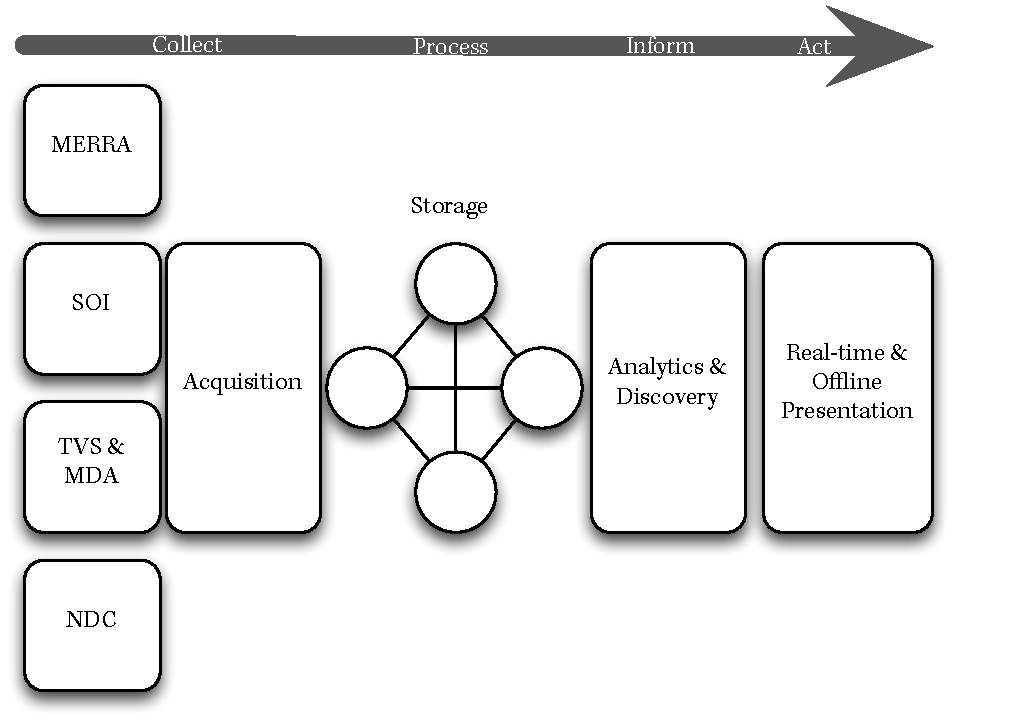
\includegraphics[scale=.75]{dataflow}
\end{figure}

\subsection{Data Acquisition}
As all the data is freely available via standard HTTP requests, we simply need to put together a framework consisting of a repeatable process that polls each website for newly published data and retrieves it. If necessary, the framework can check with the data store to confirm what's new and what's not. Putting together such a framework is a relatively simple systems integration and development task and has plenty of prior art across the industry. I'd recommend the following components:
\begin{itemize}
	\item Three Linux instances to handle retrieval, monitoring, and hosting the source code repository, respectively.
	\item A continuous integration tool, Jenkins or similar, for continually monitoring and notifying the success or failure of the retrieval processes (one per data set). Jenkins will also serve as the means to deploy the most recent code from the code repository onto the server handling the retrieval process. Jenkins is open source and used commonly across the industry for this purpose, resulting in an easily hirable skill set \cite{jenkins}.
	\item A repeatable method, such as Cron, to check and retrieve updated data sets at well defined publication intervals. Jenkins will monitor the success or failure of the cron jobs and notify as needed.
	\item Developed code that contacts each web server and pulls down only the most recent data. If the data sets do not offer a simple means of determining what's recent, this code can query the data store so that it's aware of the last stored data. While we need unique code for each data set, the process of determining what's new and retrieving the code should be very similar across all the data sets. It's likely there will a reusable common library of functionality across each specific implementation. This development is likely to be done in a scriptable environment such as Python or Perl. The languages offer an excellent tradeoff between simplicity, flexibility, and execution speed.
\end{itemize}

\subsection{Storing and Indexing}
Once the data has arrived on the local system, it needs to processed and inserted into the data store. This layer is the heart of any service offering. The data store must have the following characteristics:
\begin{itemize}
	\item Not inherently possess a single point of failure
	\item Horizontally scale (as linearly as possible) in storage and performance
	\item support realtime and batch analytics
\end{itemize}
There exist several technologies in the top level Apache Hadoop project, one being Cassandra\index{Cassandra}, which fulfill the requirements listed above\cite{cassandra}. There of competing technologies from commercial vendors like EMC, IBM, Intel, SAS, and Oracle, just to name a few, who have similar technologies designed to store and index vast amounts of data. Regardless of technology, within the data store implementation, we can use the following generic key-value model for storing any piece of climate data.
\begin{table}[htbp]
	\caption*{Climate Data Model}
	\centering
	\begin{tabular}{l l}
		\hline
		Key & Value \\ [0.5ex]
		%heading
		\hline
		meta-data & what the measurement represents, i.e., total precipitation or soil moisture\\
		time & time and date of measurement in UTC, i.e., YYYY-MM-DD HH:MM:SS\\
		coordinates & geographic location in latitude and longitude, i.e. -90.0 to 90.0 and -180.0 to 180.0\\
		value & measurement value, i.e. 0.000052977\\
		\hline
	\end{tabular}
\end{table}
With this simple structure and specific materialized views \index{materialized views}\cite{materialized_views}, we enable analytics based on any combination of the following searches: temporal, geospatial, or by meta-data.

\subsection{Discovery and Analytics}
The technology behind big data storage is really only interesting to engineers. What we want are the results of the stored data analysis. 

\subsection{Presentation}


At this point, we have a fully automated platform capable of generating predictive analytics twice a year and delivering those results electronically into an industry standard administration platform. With the future tornado probabilities by grid location, combined with the parcel and policy information, the insurance carriers now have ability to make fundamental business decisions such as: do we have enough funds to cover expected losses, do we renew policies for high probability areas, is predicted income balanced against probable risk, as well as giving another data point against fraudulent damage claims. 
